\documentclass{article}
\usepackage[utf8]{inputenc}

\usepackage{graphicx}

% Libertine for body text
\usepackage[osf]{libertine}
\linespread{1.05}
\usepackage{libertinust1math}
\usepackage[T1]{fontenc}
\usepackage[scale=0.85]{FiraMono}

\usepackage{sectsty}
\allsectionsfont{\normalfont\sffamily\bfseries}

\usepackage{microtype}

\usepackage{parskip}

\usepackage[font=sf, format=hang, labelfont=bf, labelsep=quad]{caption}

\title{TTGA -- Topological Tools for Geomorphological Analysis \\[5mm] \large Manual for version 1.4.0}
\author{}
\date{}

\begin{document}

\maketitle

TTGA is a tool which helps the analysis of river systems, in particular, braided rivers and estuaries. The focus of the tool is the computation of river networks from a digital elevation model (DEM) of the river bed. Such a river network can then be used as input for further analyses, such as computing the length or average elevation of channels.

TTGA is available for Windows and Linux systems, and is free software licensed under the GNU General Public License version 3.

\emph{Note: the current version of TTGA is an alpha version: it is not finished and is missing some features. These will be added in the future.}


\tableofcontents


\section{Workflow}

The basic workflow when using TTGA is as follows.

\begin{itemize}
    \item Prepare a DEM in either of the two input formats supported by the tool (see Section~\ref{sec:input}).
    \item Select the parameters for the river network computation (see Section~\ref{sec:parameters}).
    \item Run the computation.
    \item Either inspect the output qualitatively, or output the network to a file (see Section~\ref{sec:output}) so that a quantative analysis can be performed afterwards.
\end{itemize}

The tool provides two modes of operation. When starting the tool normally, it runs in the GUI (graphical user interface) mode (see Figure~\ref{fig:gui-start}). This mode allows setting parameters interactively, and is most suitable if you want to visually inspect the network. If the tool is started from the command line, with at least one command-line parameter, it does not start the GUI and instead runs computations as specified on the command line. This allows the program to be used from scripts. Use the \texttt{-{}-help} parameter to get an overview of all parameters available.

\begin{figure}
    \centering
    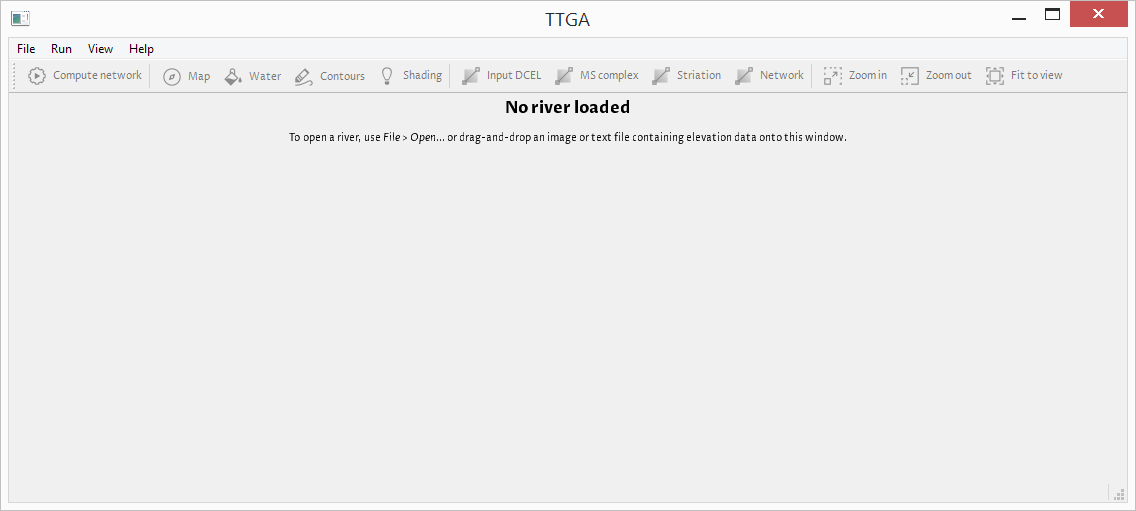
\includegraphics[width=\linewidth]{figures/gui-start.png}
    \caption{The GUI as it appears when starting the tool.}
    \label{fig:gui-start}
\end{figure}


%\section{Case study: Western Scheldt}
%\label{sec:western-scheldt}
%
%The remainder of this manual provides more technical details about how the tool works.


\section{Input formats}
\label{sec:input}

River DEMs can be supplied in two formats: a text-based format and an image-based format. The text-based format allows for more accurate elevation values and is generally recommended. The image-based format is meant only for quick experimentation, for example by drawing a fake DEM in an image editor and investigating the generated river network.

To import a DEM in either of the two formats into the tool, drag-and-drop it onto the main application window. Alteratively, use \emph{File \textgreater{} Open\ldots}.

\paragraph{Text-based format}
A text input file consists of a sequence of numbers separated by whitespace. (This whitespace separating the numbers can consist of spaces, tabs or newlines; these are irrelevant to the program)

The file starts with six numbers, determining in turn:
\begin{itemize}
\item the width of the grid (number of points in each row);
\item the height of the grid (number of points in each column);
\item the resolution in the $x$-direction (in meters per pixel);
\item the resolution in the $y$-direction (in meters per pixel);
\item the minimum height (in meters);
\item the maximum height (in meters).
\end{itemize}
After these six numbers, the height values are stored in row-major order. Each height value is just a single number. If the width and height of the grid (as given in the first two numbers in the file) are called $w$ and $h$, respectively, there need to be exactly $w \cdot h$ height values.

An example input file containing $4 \times 4$ height measurements:
\begin{verbatim}
4 4 20 20 -25 25

 -9.3 -11.8  -7.7  -7.6
-14.8 -16.9 -13.3  -9.2
 -4.5   2.3   2.6  -1.8
  6.7  20.8  13.7  11.8
\end{verbatim}

\paragraph{Image-based format}
For convenience, the program also supports loading grayscale images. Here each pixel encodes a height value: black is low and white is high. Because the resolution and minimum\,/\,maximum height cannot be contained in the image file itself, they need to be set separately (see Section~\ref{sec:parameters}). The minimum and maximum height are interpreted as the elevation of a completely black or white pixel, respectively.

In a grayscale image, only 256 distinct elevation values can be encoded (in the range 0--255). This may not be sufficient in practice. To work around this, the implementation allows another encoding of height values, namely by using the red, green and blue channels of the pixel color individually. In this scheme the height value is expressed as a 24-bit value between \texttt{0x000000} and \texttt{0xffffff}, of which the red channel stores the upper 8 bits, the green channel stores the middle 8 bits, and the blue channel stores the lower 8 bits.

\paragraph{Boundary}
By default, the program assumes that the entire rectangular DEM should be analyzed. To cut out a particular part of the DEM, it is possible to provide a boundary text file, delineating the boundary of the area to analyze.

The boundary consists of four parts, that we call \emph{source}, \emph{sink}, \emph{top} and \emph{bottom}. See Figure~\ref{fig:river-boundary}.

\begin{figure}
    \centering
    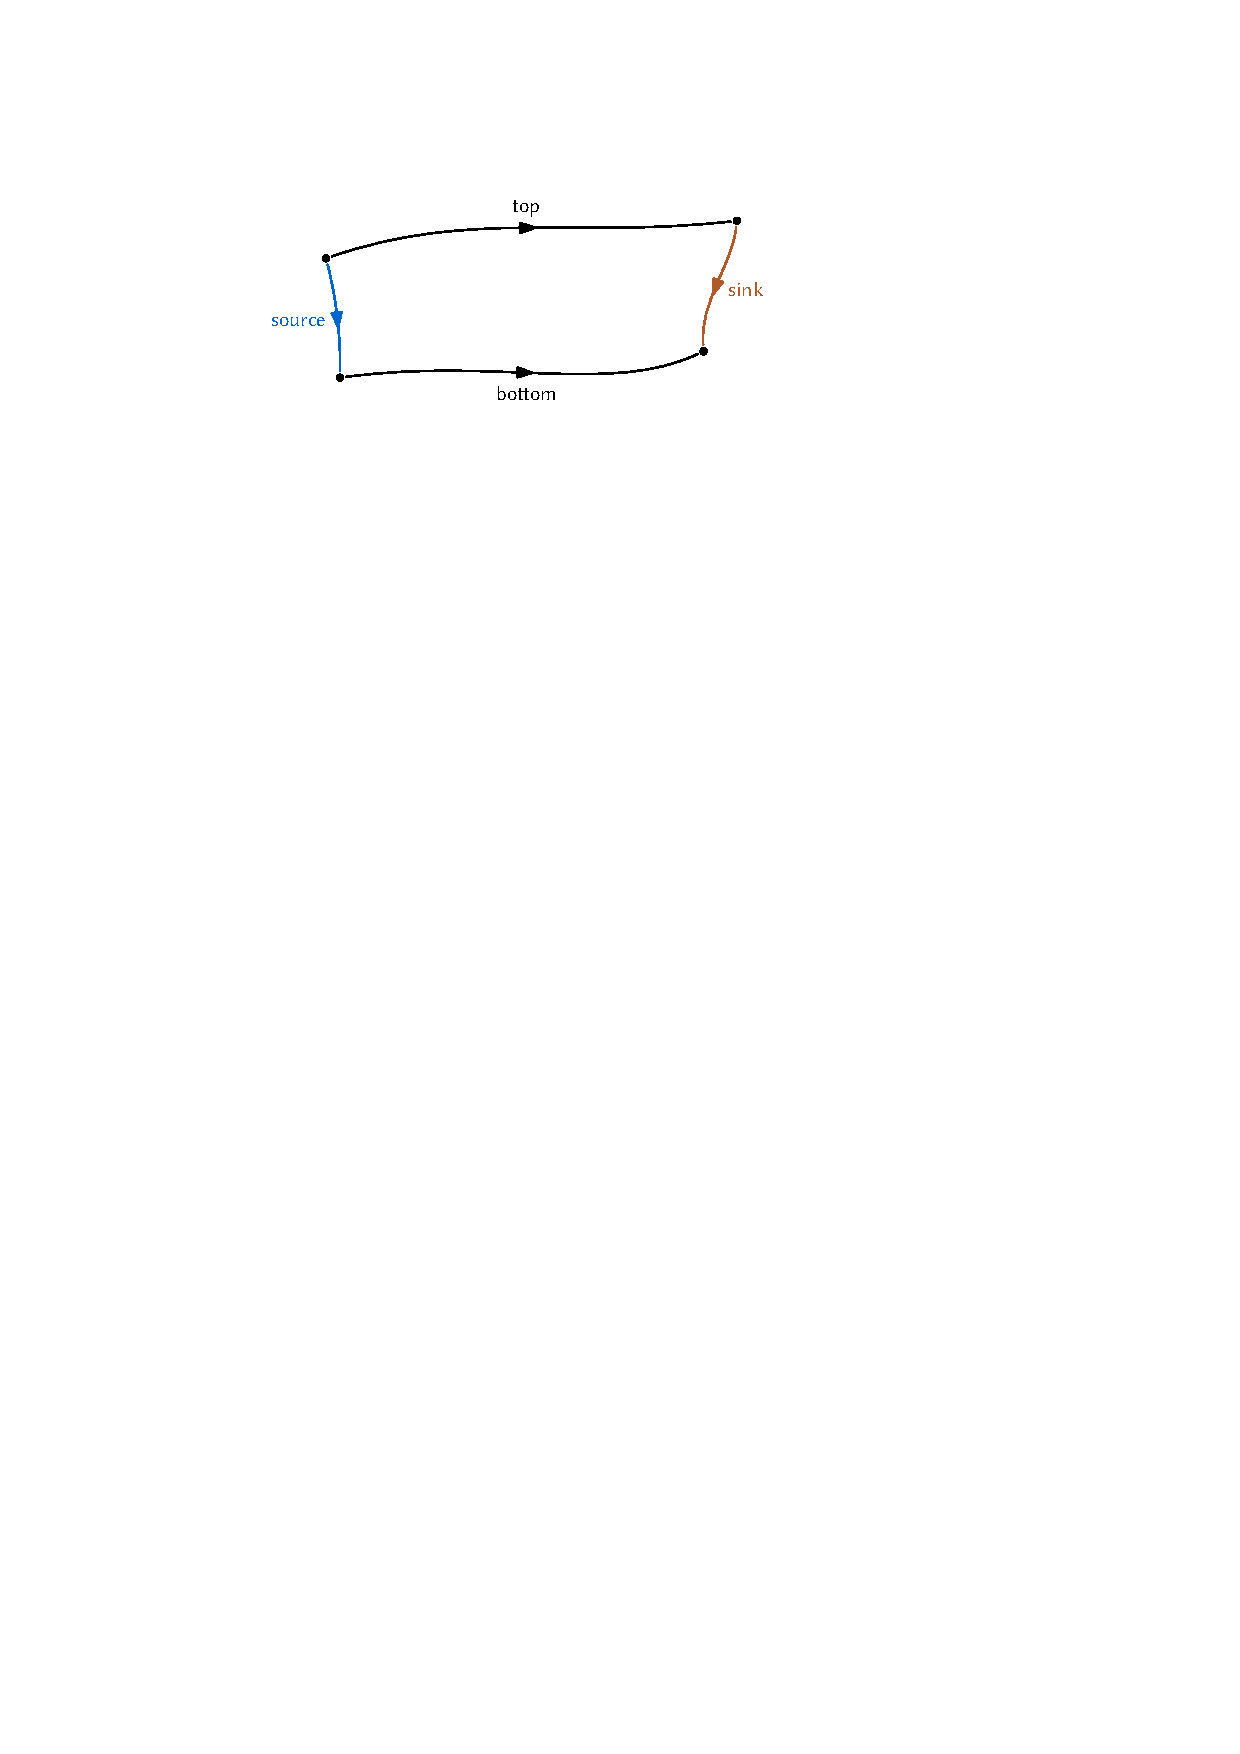
\includegraphics{figures/river-boundary}
    \caption{The four parts of a river boundary.}
    \label{fig:river-boundary}
\end{figure}

The exact format of a boundary text file is as follows. It is a normal text file containing numbers (just like the text-based DEM format), starting with four numbers giving the length (number of vertices) of the source, sink, top and bottom paths, in that order. Then, the source path is given as an ordered list of points (each point is given as two numbers: its $x$- and $y$-coordinate), followed by the sink path, the top path and the bottom path, in that order.

The boundary must meet a number of requirements. No coordinate may be included in the boundary twice, and of course the coordinates are not allowed to go outside the boundary of the rectangular DEM itself. (That is, if your DEM is $10 \times 10$, the coordinates in the boundary file need to stay within the range $0$--$10$.) Furthermore each segment of each path needs to be a horizontal or vertical, with length~$1$. The program shows an error message if the given boundary is incorrect.

An example boundary file:
\begin{verbatim}
3 2 4 3

1 1    1 2    1 3
3 2    3 3
1 1    2 1    2 2    3 2
1 3    2 3    3 3
\end{verbatim}

\emph{Note: we are working on adding a boundary editor to the tool itself, so it will not be necessary anymore to create a boundary file by hand.}


\section{Parameter choices}
\label{sec:parameters}

The tool implements two separate algorithms for computing the river network: the (older) \emph{striation-based algorithm} and the (newer) \emph{persistence-based algorithm}. The persistence-based algorithm is selected by default, and in fact we recommend that the persistence-based algorithm be used for all analyses, as it is more stable. That is, minor changes in the DEM have only a local influence in the generated river network, as opposed to potentially changing the entire network. The persistence-based algorithm also requires fewer parameters to be set manually. For this reason, the striation-based algorithm will likely be removed in a future version of the tool.

\begin{figure}
    \centering
    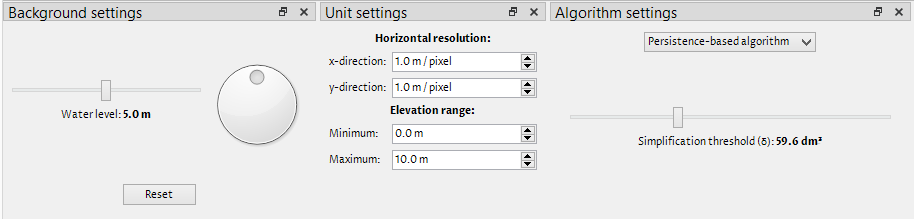
\includegraphics[width=\linewidth]{figures/parameters.png}
    \caption{The interface for setting parameters for the computation.}
    \label{fig:parameters}
\end{figure}

As soon as a DEM has been loaded into the tool, an interface for setting parameters becomes visible (see Figure~\ref{fig:parameters}). After setting the parameters, the computation can be run by clicking \emph{Compute network}. While the computation is running, progress information is visible in the \emph{Progress viewer} area on the right.

The following parameters can be modified.

\paragraph{Background settings}
With these controls, the water level and slope of the river can be set. Note that these parameters do \emph{not} influence the resulting river network at all: they modify only the river display in the tool itself. For this reason, these parameters cannot be modified in the command-line interface. The \emph{Reset} button resets these parameters to their default values.

\paragraph{Unit settings}
Here the horizontal resolution and elevation range can be set. In case the text-based input format was used (see Section~\ref{sec:input}), these parameters are simply taken from the file. They can however still be overridden here, if necessary. In case the image-based input format was used, the parameters are set to default values and should be changed to correspond to the physical reality.

In the command-line mode, these parameters can be set using the \texttt{-{}-xRes}, \texttt{-{}-yRes}, \texttt{-{}-minHeight}, and \texttt{-{}-maxHeight} command-line options.

\paragraph{Algorithm settings}
In this part of the interface, the algorithm can be fine-tuned. In the dropdown, the striation-based or the persistence-based algorithm can be chosen.

In the command-line mode, the algorithm can be set by \texttt{-{}-algorithm striation} or \texttt{-{}-algorithm persistence}.

The most important~-- and in case of the persistence-based algorithm, the only~-- parameter is the simplification threshold~$\delta$. This setting controls how many channels are included in the network. The smaller the threshold~$\delta$ is, the more channels remain. When $\delta$ becomes larger, the least significant channels disappear. When using the persistence-based algorithm, $\delta$ does not need to be set before running the computation. Instead, after the computation has finished, $\delta$ can be changed while the displayed network changes interactively.

In the command-line mode, the simplification threshold can be set using the \texttt{-{}-delta} option. This option takes a list of one or more values, separated by semicolons. If more than one value is provided, the computation is run and a network is exported for all values individually.


\section{Output formats}
\label{sec:output}

The tool can export to two formats: a graph or a link sequence. Of these, the link sequence is likely to be the most useful for further analysis.

\paragraph{Link sequence}
A link sequence is a representation of a river network that consists of an ordered list of \emph{links}. A link is a path representing a river channel. Each link has an associated significance value that indicates how significant the channel is. More formally, link~$l$ has significance $\text{sig}_l$ if it appears in each river network computed with $\delta < \text{sig}_l$, and does not appear in each network with $\delta > \text{sig}_l$.

Links are sorted by ascending significance values. The first link, with infinite significance, starts at the source and ends at the sink. Each subsequent link starts and ends at some point on a link before it.

The first line of the file contains a number, indicating how many links there are. The remainder of the file has one line for each link. Such a line contains an identifier (counting upwards from~$0$), then the significance value, and then a sequence of points ($x$- and $y$-coordinates).

An example output file containing one link:
\begin{verbatim}
1
0 inf -1 2 1 1 2 1 2 2 3 2 4 2
\end{verbatim}

Note that the link in this file starts at coordinate $(-1, 2)$, which is the source. It ends at $(4, 2)$, which is the sink.

\end{document}
